%
% This presentation is for use at the MDACC Medical Physics Trainee 2015 Summer
% Seminar Series on July 6, 2015.
%

\documentclass{beamer}
\usepackage{amsmath}
\usepackage{graphicx}
\usetheme{Warsaw}
\graphicspath{{Images/}}

%%%%%%%%%%%%%%%%%%%%%%%%%%%%%%%%%%%%%%%%%%%%%%%%%%%%%%%%%%%%%%%%%%%%%%%%%%%
% Title Page
%%%%%%%%%%%%%%%%%%%%%%%%%%%%%%%%%%%%%%%%%%%%%%%%%%%%%%%%%%%%%%%%%%%%%%%%%%%
\title[Spinal Cord DWI with ss-EPI]{DWI of the Spinal Cord with Reduced FOV Single-Shot EPI}
\author{Drew Mitchell}
\institute{MD Anderson Cancer Center}
\date{June 17, 2015}
%\AtBeginSection[]
%{{
%\setbeamertemplate{headline}{}
%\frame{\tableofcontents[currentsection]}
%}}

\begin{document} 
{
\setbeamertemplate{headline}{}
\frame{\titlepage}
\begin{frame}{Table of Contents}
\tableofcontents
\end{frame}
}

%%%%%%%%%%%%%%%%%%%%%%%%%%%%%%%%%%%%%%%%%%%%%%%%%%%%%%%%%%%%%%%%%%%%%%%%%%%
% Introduction
%%%%%%%%%%%%%%%%%%%%%%%%%%%%%%%%%%%%%%%%%%%%%%%%%%%%%%%%%%%%%%%%%%%%%%%%%%%
\section{Introduction}

\begin{frame}{Introduction}
\begin{itemize}
	\item Spinal cord diffusion-weighted imaging (DWI) can diagnose disorders from fiber tract damage
	\item Several challenges:
	\begin{itemize}
		\item Magnetic field inhomogeneities around spine create off-resonance artifacts
		\item Partial volume effects from CSF and lipid
		\item Spinal cord cross section very small
		\item Bulk physiologic motion from heart, breathing, swallowing, CSF pulsation
	\end{itemize}
	\item Result is low-signal, low-resolution DW images with artifacts in spinal cord
\end{itemize}
\end{frame}

\begin{frame}{Introduction}
\begin{itemize}
	\item Single-shot echo planar imaging (ss-EPI) most frequently used technique for DWI
	\begin {itemize}
		\item Acquires whole k-space after single excitation pulse
		\item No ghosting artifacts from motion-induced phase errors
	\end {itemize}
	\item Long readout experiences $T_2^*$ decay
\end{itemize}
\end{frame}

\begin{frame}{Introduction}
\begin{itemize}
	\item Spinal cord imaging benefits from reduced FOV applications
	\item Reduced FOV methods decrease the readout duration and reduce off-resonance artifacts
	\item Excited FOV in PE direction reduced by 2D spatially selective echo-planar RF excitation pulse and $180^{\circ}$ refocusing RF pulse
	\item Allows multi slice imaging and suppresses fat signal
\end{itemize}
\end{frame}
	
%%%%%%%%%%%%%%%%%%%%%%%%%%%%%%%%%%%%%%%%%%%%%%%%%%%%%%%%%%%%%%%%%%%%%%%%%%%
% Theory
%%%%%%%%%%%%%%%%%%%%%%%%%%%%%%%%%%%%%%%%%%%%%%%%%%%%%%%%%%%%%%%%%%%%%%%%%%%
\section{Theory}

\begin{frame}{Theory}
\begin{columns}[T]
	\begin{column}[T]{5cm}
		Standard DW spin-echo ss-EPI sequence, with excitation pulse replaced with $90^{\circ}$ 2D spatially selective echo-planar RF pulse
	\end{column}
	\begin{column}[T]{5cm}
		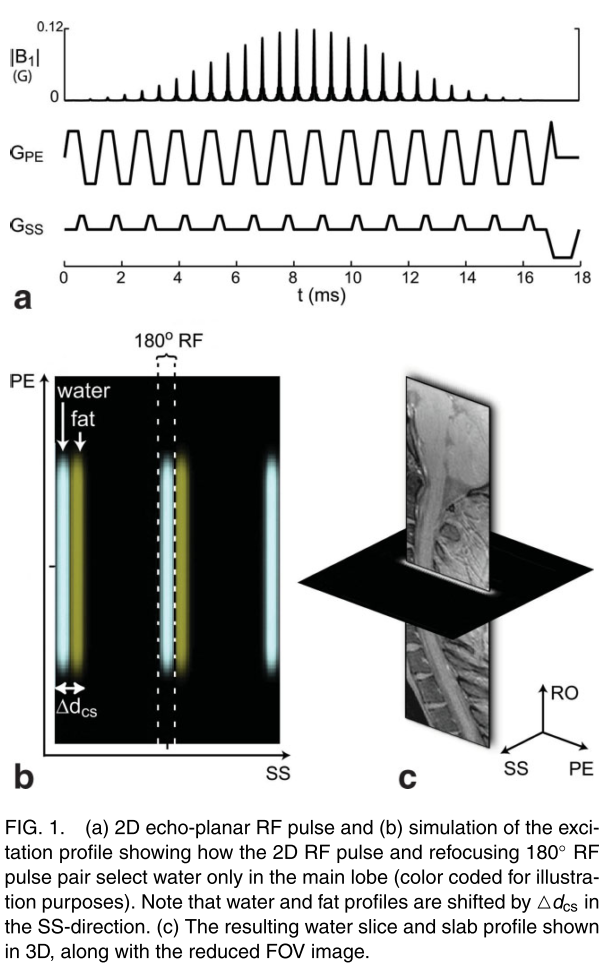
\includegraphics[height=6cm]{SpineDWIfig1}
	\end{column}
\end{columns}
\end{frame}

\subsection{2D Echo-Planar RF Pulse}

\begin{frame}{2D Echo-Planar RF Pulse}

\end{frame}

\subsection{Multi Slice Imaging}

\begin{frame}{Multi Slice Imaging}

\end{frame}

%%%%%%%%%%%%%%%%%%%%%%%%%%%%%%%%%%%%%%%%%%%%%%%%%%%%%%%%%%%%%%%%%%%%%%%%%%%
% Methods
%%%%%%%%%%%%%%%%%%%%%%%%%%%%%%%%%%%%%%%%%%%%%%%%%%%%%%%%%%%%%%%%%%%%%%%%%%%
\section{Methods}
\subsection{Phantom Experiments}
\subsection{In Vivo Imaging}
\subsection{Image Reconstruction}

%%%%%%%%%%%%%%%%%%%%%%%%%%%%%%%%%%%%%%%%%%%%%%%%%%%%%%%%%%%%%%%%%%%%%%%%%%%
% Results
%%%%%%%%%%%%%%%%%%%%%%%%%%%%%%%%%%%%%%%%%%%%%%%%%%%%%%%%%%%%%%%%%%%%%%%%%%%
\section{Results}
\subsection{Phantom Experiment Results}
\subsection{In Vivo Imaging Results}

%%%%%%%%%%%%%%%%%%%%%%%%%%%%%%%%%%%%%%%%%%%%%%%%%%%%%%%%%%%%%%%%%%%%%%%%%%%
% Discussion
%%%%%%%%%%%%%%%%%%%%%%%%%%%%%%%%%%%%%%%%%%%%%%%%%%%%%%%%%%%%%%%%%%%%%%%%%%%
\section{Discussion}

%\begin{frame}{Discussion}
%
%\end{frame}

\subsection{Fat Suppression}
\subsection{Image Reconstruction}

\begin{frame}{test}
\end{frame}
\end{document}

